%% For normal draft builds (figs undisplayed hence fast compile)
%\documentclass[hyperpdf,nobind,draft,oneside]{hepthesis}
%\documentclass[hyperpdf,nobind,draft,twoside]{hepthesis}

%% For short draft builds (breaks citations by necessity)
%\documentclass[hyperpdf,nobind,draft,hidefrontback]{hepthesis}

%%For Cambridge soft-bound version
\documentclass[hyperpdf,bindnopdf]{hepthesis}
%% For Cambridge hard-bound version (must be one-sided)
%\documentclass[hyperpdf,oneside]{hepthesis}

%% Load special font packages here if you wish
%\usepackage{lmodern}
\usepackage{mathpazo}
%\usepackage{euler}

%% Put package includes etc. into preamble.tex for convenience
\newcommand\hmmax{0}
\newcommand\bmmax{0}
\usepackage{xspace}
%\usepackage{tikz}
\usepackage{morefloats,afterpage}%\usepackage{subfig}
\usepackage{mathrsfs} % script font
\usepackage{verbatim}
\usepackage{amssymb}
\usepackage{tabularx}
%\usepackage{mathtools}
%\usepackage{caption}
\usepackage{subcaption}
\usepackage{epstopdf}
\usepackage{multirow}
\epstopdfsetup{update}

%\usepackage{CJKutf8}
%\AtBeginDvi{\input{zhwinfonts}}
%% Using Babel allows other languages to be used and mixed-in easily
%\usepackage[ngerman,english]{babel}
\usepackage[british]{babel}
\selectlanguage{british}

%% Citation system tweaks
\usepackage{cite}
% \let\@OldCite\cite
% \renewcommand{\cite}[1]{\mbox{\!\!\!\@OldCite{#1}}}

\renewcommand*{\figureformat}{\figurename~\thefigure}
\renewcommand*{\tableformat}{\tablename~\thetable}
\renewcommand{\autodot}{}% Remove all end-of-counter dots

\DeclareOldFontCommand{\rm}{\normalfont\rmfamily}{\mathrm}
\DeclareOldFontCommand{\sf}{\normalfont\sffamily}{\mathsf}
\DeclareOldFontCommand{\tt}{\normalfont\ttfamily}{\mathtt}
\DeclareOldFontCommand{\bf}{\normalfont\bfseries}{\mathbf}
\DeclareOldFontCommand{\it}{\normalfont\itshape}{\mathit}
\DeclareOldFontCommand{\sl}{\normalfont\slshape}{\@nomath\sl}
\DeclareOldFontCommand{\sc}{\normalfont\scshape}{\@nomath\sc}
\DeclareRobustCommand*\cal{\@fontswitch\relax\mathcal}
\DeclareRobustCommand*\mit{\@fontswitch\relax\mathnormal}

\newcolumntype{R}[1]{>{\raggedleft\arraybackslash}p{#1}}
\newcolumntype{L}[1]{>{\raggedright\arraybackslash}p{#1}}

\newenvironment{myfont}{\fontfamily{cmr}\selectfont}{\par}
\DeclareTextFontCommand{\textmyfont}{\myfont}
%% Maths
% TODO: rework or eliminate maybemath
\usepackage{abmath}


\DeclareRobustCommand{\mymath}[1]{\ensuremath{\maybebmsf{#1}}}
\DeclareRobustCommand{\uprightMath}[1]{\MathUpright{\mymath{#1}}}

\DeclareRobustCommand{\Rate}{\mymath{\Gamma}\xspace}
\DeclareRobustCommand{\RateOf}[1]{\mymath{\Gamma}\parenths{#1}\xspace}

\DeclareRobustCommand{\Table}[1]{table \ref{#1}\xspace}
\DeclareRobustCommand{\TABLE}[1]{Table \ref{#1}\xspace}
\DeclareRobustCommand{\Section}[1]{section \ref{#1}\xspace}
\DeclareRobustCommand{\SECTION}[1]{Section \ref{#1}\xspace}
\DeclareRobustCommand{\Chapter}[1]{chapter \ref{#1}\xspace}
\DeclareRobustCommand{\CHAPTER}[1]{Chapter \ref{#1}\xspace}
\DeclareRobustCommand{\Figure}[1]{figure \ref{#1}\xspace}
\DeclareRobustCommand{\FIGURE}[1]{Figure \ref{#1}\xspace}
\DeclareRobustCommand{\Equation}[1]{equation \ref{#1}\xspace}
\DeclareRobustCommand{\EQUATION}[1]{Equation \ref{#1}\xspace}
\DeclareRobustCommand{\Reference}[1]{reference \cite{#1}\xspace}
\DeclareRobustCommand{\REFERENCE}[1]{Reference \cite{#1}\xspace}
%% High-energy physics stuff
\usepackage{abhep}
\usepackage{hepnames}
\usepackage{hepunits}

\newlength{\widthOne}
\setlength{\widthOne}{12cm}

\DeclareRobustCommand{\SM}{SM\xspace}
\DeclareRobustCommand{\QED}{QED\xspace}
\DeclareRobustCommand{\QCD}{QCD\xspace}

\DeclareMathOperator{\Lagr}{\mathcal{L}}
\DeclareRobustCommand{\Dstroke}{\mymath{\gamma^{\mu}D_{\mu}}\xspace}
\DeclareRobustCommand{\Hmass}{\mymath{m_{\PH}}\xspace}

\DeclareRobustCommand{\Guineapig}{\textsc{GuineaPig}\xspace}
\DeclareRobustCommand{\Zqq}{\HepProcess{ \PZ \to \Pquark\Pquark}\xspace}
\DeclareRobustCommand{\Wqq}{\HepProcess{ \PW \to \Pquark\Pquark}\xspace}

%\DeclareRobustCommand{\charge}{\HepParticle{X}{}{\pm}\xspace}
%\DeclareRobustCommand{\neutral}{\HepParticle{X}{}{0}\xspace}
\DeclareRobustCommand{\charge}{C}
\DeclareRobustCommand{\neutral}{N}
\DeclareRobustCommand{\weinberg}{\uprightMath{\theta_{\PW}}}

\DeclareRobustCommand{\PhotonReconstruction}{\textsc{Photon Reconstruction}\xspace}
\DeclareRobustCommand{\ShowerPeak}{\textsc{Shower Peak}\xspace}
\DeclareRobustCommand{\peakFinding}{\textsc{2D Peak Finding}\xspace}
\DeclareRobustCommand{\multiclass}{\textsc{MultiClass}\xspace}
\DeclareRobustCommand{\DoPreSelection}{\textsc{DoPreSelection}\xspace}


\DeclareRobustCommand{\RM}{Moli\`{e}re radius\xspace}
\DeclareRobustCommand{\rms}{root-mean-square\xspace}

\DeclareRobustCommand{\Zprime}{\HepParticle{Z}{}{\prime}\xspace}
\DeclareRobustCommand{\Zuds}{\HepProcess{ \Zprime \to \Pup\APup/\Pdown\APdown/\Pstrange\APstrange}\xspace}
\DeclareRobustCommand{\eeZuds}{\HepProcess{ \Pep \Pem \to \Zprime\Zprime}\xspace samples, where \Zuds}
\DeclareRobustCommand{\ISR}{ISR\xspace}
\DeclareRobustCommand{\FSR}{FSR\xspace}

\DeclareRobustCommand{\myDagger}{\mymath{\dagger}\xspace}

\DeclareRobustCommand{\TauTau}{\HepProcess{\APtauon\Ptauon}\xspace}
\DeclareRobustCommand{\TauTauSub}[2]{\HepProcess{\HepParticle{\tau}{#1}{+}\xspace\HepParticle{\tau}{#2}{-}\xspace}\xspace}
\DeclareRobustCommand{\TauFull}[2]{\HepParticle{\tau}{#1}{#2}\xspace}

\DeclareRobustCommand{\MuMu}{\HepProcess{ \APmuon\Pmuon}\xspace}

\DeclareRobustCommand{\HigssTauTau}{\HepProcess{\PHiggs\APtauon\Ptauon}\xspace}
\DeclareRobustCommand{\ZTauTau}{\HepProcess{\PZ\APtauon\Ptauon}\xspace}
\DeclareRobustCommand{\ZToqq}{\HepProcess{\PZ\to\Pquark\Pquark}\xspace}
\DeclareRobustCommand{\HiggsToTauTau}{\HepProcess{\PHiggs \to \APtauon \Ptauon}\xspace}
\DeclareRobustCommand{\ZToTauTau}{\HepProcess{\PZ \to \APtauon \Ptauon}\xspace}
\DeclareRobustCommand{\eeZZ}{\HepProcess{\Pep \Pem \to \PZ\PZ}\xspace}
\DeclareRobustCommand{\eeHZ}{\HepProcess{\Pep \Pem \to \PHiggs\PZ}\xspace}
\DeclareRobustCommand{\eeTauTau}{\HepProcess{\Pep \Pem \to \APtauon\Ptauon}\xspace}
\DeclareRobustCommand{\eeZZQQ}{\HepProcess{\Pep \Pem \to \PZ\PZ \to \APtauon\Ptauon \Pquark\Pquark }\xspace}
\DeclareRobustCommand{\eeHZQQ}{\HepProcess{\Pep \Pem \to \PHiggs\PZ \to \APtauon\Ptauon \Pquark\Pquark }\xspace}


%\DeclareRobustCommand{\charge}{\HepParticle{\chi}{}{+}\xspace}
%\DeclareRobustCommand{\neutral}{\HepParticle{\chi}{}{0}\xspace}
\DeclareRobustCommand{\Pai}{\HepParticle{a}{1}{}\xspace}
\DeclareRobustCommand{\tauToPion}{\HepProcess{\Ptauon \to \Pgpm\Pgngt}\xspace}
\DeclareRobustCommand{\tauToPionBoth}{\HepProcess{\Ptaupm \to \Pgppm\Pgngt}\xspace}
\DeclareRobustCommand{\pionToPhoton}{\HepProcess{\Ppizero \to \Pgamma \Pgamma}\xspace}
\DeclareRobustCommand{\decayElectron}{\HepProcess{\Pem\Pagne\Pgngt}\xspace}
\DeclareRobustCommand{\decayMuon}{\HepProcess{\Pgmm\Pagngm\Pgngt}\xspace}
\DeclareRobustCommand{\decayPion}{\HepProcess{\Pgpm\Pgngt}\xspace}
\DeclareRobustCommand{\decayRhoFinalState}{\HepProcess{\Pgpm\Ppizero\Pgngt}\xspace}
\DeclareRobustCommand{\decayRhoFinalStateShort}{\HepProcess{\Pgpm\Ppizero}\xspace}

\DeclareRobustCommand{\tauToElectron}{\HepProcess{\Ptauon \to \Pem\Pagne\Pgngt}\xspace}
\DeclareRobustCommand{\tauToMuon}{\HepProcess{\Ptauon \to \Pgmm\Pagngm\Pgngt}\xspace}
\DeclareRobustCommand{\tauToRho}{\HepProcess{\Ptauon \to \decayRhoShort\Pgngt}\xspace}
\DeclareRobustCommand{\tauToAiPhoton}{\HepProcess{\Ptauon \to \decayAiPhotonShort\Pgngt}\xspace}
\DeclareRobustCommand{\tauToAiPion}{\HepProcess{\Ptauon \to \decayAiPionShort\Pgngt}\xspace}


\DeclareRobustCommand{\decayRho}{\HepProcess{\rho\Pgngt}\xspace}
\DeclareRobustCommand{\decayAi}{\HepProcess{a_1\Pgngt}\xspace}
\DeclareRobustCommand{\decayAiPhoton}{\HepParticleResonanceFull{a}{1}{}{\Pgpm\Pgpz\Pgpz}{}{}\Pgngt\xspace}
\DeclareRobustCommand{\decayAiPhotonFinalState}{\HepProcess{\Pgpm\Pgpz\Pgpz\Pgngt}\xspace}
\DeclareRobustCommand{\decayAiPhotonFinalStateShort}{\HepProcess{\Pgpm\Pgpz\Pgpz}\xspace}
\DeclareRobustCommand{\decayAiPion}{\HepParticleResonanceFull{a}{1}{}{\Pgpm\Pgpm\Pgpp}{}{}\Pgngt\xspace}
\DeclareRobustCommand{\decayAiPionFinalState}{\HepProcess{\Pgpp\Pgpm\Pgpm\Pgngt}\xspace}
\DeclareRobustCommand{\decayAiPionFinalStateShort}{\HepProcess{\Pgpp\Pgpm\Pgpm}\xspace}

\DeclareRobustCommand{\decayThreePionPhoton}{\HepProcess{\Pgpp\Pgpm\Pgpm\Pgpz\Pgngt}\xspace}

\DeclareRobustCommand{\tauToThreePion}{\HepProcess{\Ptauon \to \decayThreePionPhoton}\xspace}

\DeclareRobustCommand{\decayElectronShort}{\Pem\xspace}
\DeclareRobustCommand{\decayMuonShort}{\Pgmm\xspace}
\DeclareRobustCommand{\decayPionShort}{\Pgpm\xspace}


\DeclareRobustCommand{\decayRhoShort}{\HepParticleResonance{\rho}{\Pgpm\Ppizero}{}{}\xspace}
\DeclareRobustCommand{\decayAiPhotonShort}{\HepParticleResonanceFull{a}{1}{}{\Pgpm\Pgpz\Pgpz}{}{}\xspace}
\DeclareRobustCommand{\decayAiPionShort}{\HepParticleResonanceFull{a}{1}{}{\Pgpp\Pgpm\Pgpm}{}{}\xspace}
\DeclareRobustCommand{\decayThreePionPhotonShort}{\HepProcess{\Pgpp\Pgpm\Pgpm\Pgpz}\xspace}

\DeclareRobustCommand{\eeToTauTau}{\HepProcess{ \Pep \Pem \to \Pgtp \Pgtm }\xspace}

\DeclareRobustCommand{\decayRhoShortest}{\HepParticleResonance{\rho}{\Pgpm\Ppizero}{}{}\xspace}
\DeclareRobustCommand{\decayAiPhotonShortest}{\HepParticleResonanceFull{a}{1}{}{\Pgpm\Pgpz\Pgpz}{}{}\xspace}
\DeclareRobustCommand{\decayAiPionShortest}{\HepParticleResonanceFull{a}{1}{}{\Pgpp\Pgpm\Pgpm}{}{}\xspace}
\DeclareRobustCommand{\tauHad}{\mymath{\varepsilon_{had}}\xspace}



\DeclareRobustCommand{\PhotonFragmentRemoval}{\textsc{PhotonFragmentRemoval}\xspace}
\DeclareRobustCommand{\ClosestHitDistance}{\textsc{ClosestHitDistance}\xspace}

\DeclareRobustCommand{\gHHH}{\HepParticle{g}{HHH}{}\xspace}
\DeclareRobustCommand{\gWWH}{\HepParticle{g}{WWH}{}\xspace}
\DeclareRobustCommand{\gWWHH}{\HepParticle{g}{WWHH}{}\xspace}
\DeclareRobustCommand{\gHHHSM}{\HepParticle{g}{HHH}{SM}\xspace}
\DeclareRobustCommand{\gWWHHSM}{\HepParticle{g}{WWHH}{SM}\xspace}
\DeclareRobustCommand{\rootS}[1]{\sqrtS = #1\,TeV\xspace}
\DeclareRobustCommand{\rootSGeV}[1]{\sqrtS = #1\,GeV\xspace}
\DeclareRobustCommand{\ee}{\HepProcess{ \Pep\Pem}\xspace}
\DeclareRobustCommand{\Egamma}{\HepProcess{ \Pepm\Pgamma}\xspace}
\DeclareRobustCommand{\gammae}{\HepProcess{ \Pgamma\Pepm}\xspace}
\DeclareRobustCommand{\Gammagamma}{\HepProcess{ \Pgamma\Pgamma}\xspace}
\DeclareRobustCommand{\BS}{\text{BS}\xspace}
\DeclareRobustCommand{\EPA}{\text{EPA}\xspace}

\DeclareRobustCommand{\BonoTauFinder}{\textsc{IsolatedTauIdentifer}\xspace}
\DeclareRobustCommand{\BonoLeptonFinder}{\textsc{IsolatedLeptonIdentifer}\xspace}
\DeclareRobustCommand{\IsolatedLeptonFinderProcessor}{\textsc{IsolatedLeptonFinder}\xspace}
\DeclareRobustCommand{\TauFinderProcessor}{\textsc{TauFinder}\xspace}

 \DeclareRobustCommand{\WW}{\HepProcess{\PWplus\PWminus}\xspace}
\DeclareRobustCommand{\eeToHH}{\HepProcess{ \Pep \Pem \to \PHiggs \PHiggs \Pnue \APnue }\xspace}
\DeclareRobustCommand{\bbWW}{\HepProcess{ \Pbottom \APbottom \PWplus \PWminus}\xspace}
\DeclareRobustCommand{\bbbb}{\HepProcess{ \Pbottom \Pbottom \APbottom  \APbottom }\xspace}
\DeclareRobustCommand{\eeToHHbbWW}{\HepProcess{ \PHiggs \PHiggs \to \Pbottom \APbottom \PWplus \PWminus}\xspace}
\DeclareRobustCommand{\eeToHHbbqqqq}{\HepProcess{ \PHiggs \PHiggs \to \Pbottom \APbottom \Pq \Pq \Pq \Pq}\xspace}
\DeclareRobustCommand{\eeToHHbbWWFull}{\HepProcess{ \Pep \Pem \to \PHiggs \PHiggs \Pnue \APnue \to \Pbottom \APbottom \PWplus \PWminus}\xspace}
\DeclareRobustCommand{\eeToHHbbWWHad}{\HepProcess{ \PHiggs \PHiggs \to \Pbottom \APbottom \PWplus \PWminus \to \Pbottom \APbottom \Pq \Pq \Pq \Pq}\xspace}
\DeclareRobustCommand{\eeToHHbbWWHadFull}{\HepProcess{ \PHiggs \PHiggs \Pnue \APnue \to \Pbottom \APbottom \PWplus \PWminus  \Pnue \APnue \to \Pbottom \APbottom \Pquark \Pquark \Pquark \Pquark \Pnue \APnue}\xspace}
\DeclareRobustCommand{\HHvv}{\HepProcess{\PHiggs \PHiggs \Pnue \APnue }\xspace}

\DeclareRobustCommand{\eeToHHbbbb}{\HepProcess{ \PHiggs \PHiggs \to \Pbottom \APbottom \Pbottom \APbottom}\xspace}
\DeclareRobustCommand{\eeToHHbbbbFull}{\HepProcess{\Pep \Pem \to  \PHiggs \PHiggs  \Pnue \APnue \to \Pbottom \APbottom \Pbottom \APbottom  \Pnue \APnue}\xspace}
\DeclareRobustCommand{\eeToHHotherFull}{\HepProcess{\Pep \Pem \to  \PHiggs \PHiggs \to \text{others}}\xspace}
\DeclareRobustCommand{\eeTo}[1]{\HepProcess{ \Pep \Pem \to #1 }\xspace}
\DeclareRobustCommand{\ggHad}{\HepProcess{ \Pphoton \Pphoton \to \text{hadrons} }\xspace}

\DeclareRobustCommand{\qlight}{\HepGenParticle{q}{l}{}\xspace}
\DeclareRobustCommand{\Aqlight}{\HepGenAntiParticle{q}{l}{}\xspace}
\DeclareRobustCommand{\llight}{\HepGenParticle{l}{l}{}\xspace}
\DeclareRobustCommand{\egamma}[4]{\HepProcess{ #1 #2 (#3) \to #4}\xspace}
\DeclareRobustCommand{\gammagamma}[5]{\HepProcess{ #1 (#2) #3 (#4) \to #5}\xspace}

\DeclareRobustCommand{\cosTheta}{\mymath{\cos(\MathUpright{\theta})}\xspace}
\DeclareRobustCommand{\absCosTheta}{\mymath{\lvert\cos(\MathUpright{\theta}_{\MathUpright{Z}})\rvert}\xspace}
\DeclareRobustCommand{\rZero}{\mymath{r_{0}}\xspace}
\DeclareRobustCommand{\kt}{\mymath{k_{t}}\xspace}
\DeclareRobustCommand{\y}[1]{\mymath{y_{#1}}\xspace}
\DeclareRobustCommand{\btag}{\mymath{B}\xspace}
\DeclareRobustCommand{\btagFull}[1]{\mymath{B_{#1}}\xspace}
\DeclareRobustCommand{\sumBtag}[1]{\mymath{\Sigma{\btag}_{#1\xspace{jets}}}\xspace}
\DeclareRobustCommand{\partialSumBtag}[3]{\mymath{\sum_{#1}^{#2}{\btag}_{#3\!{\text{jets}}}}\xspace}
\DeclareRobustCommand{\ctagFull}[1]{\mymath{C_{#1}}\xspace}
\DeclareRobustCommand{\sphericity}{\mymath{\textbf{S}}\xspace}
\DeclareRobustCommand{\abs}[1]{\mods{#1}}
\DeclareRobustCommand{\acolinearity}[1]{\mymath{\textit{A}_{#1}}\xspace}
\DeclareRobustCommand{\npfo}[1]{\mymath{N_{#1}}\xspace}
\DeclareRobustCommand{\cosStar}[1]{\mymath{\cosOf{\theta^{*}_{#1}}}\xspace}
\DeclareRobustCommand{\rootOf}[1]{\mymath{\sqrt{#1}}\xspace}

\DeclareRobustCommand{\W*}{\HepParticle{W}{}{*}\xspace}
\DeclareRobustCommand{\Hbb}{\HepParticle{H}{\Pbottom\Pbottom}{}\xspace}
\DeclareRobustCommand{\HWW}{\HepParticle{H}{\PW\W*}{}\xspace}
\DeclareRobustCommand{\HH}{\HepParticle{HH}{}{}\xspace}

\DeclareRobustCommand{\mhh}{\mymath{m_{\HH}}\xspace}
\DeclareRobustCommand{\HT}{\mymath{H_T}\xspace}

\DeclareRobustCommand{\HiggsTableFull}[2]{Table shows the signal and background events at \rootS{#1}, assuming an integrated luminosity of #2\,\uprightMath{fb^{-1}}. \Pquark can be \Pup, \Pdown, \Pstrange, \Pbottom or \Ptop. Unless specified, \Pquark, \Plepton and \Pnu represent either particles or the corresponding anti-particles.}

\DeclareRobustCommand{\HiggsTableLow}{\HiggsTableFull{1.4}{1500}}
\DeclareRobustCommand{\HiggsTableHigh}{\HiggsTableFull{3}{2000}}

\DeclareRobustCommand{\loosePFO}{loose selected PFO collection\xspace}
\DeclareRobustCommand{\normalPFO}{selected PFO collection\xspace}
\DeclareRobustCommand{\tightPFO}{tight selected PFO collection\xspace}
\DeclareRobustCommand{\LoosePFO}{Loose selected PFO collection\xspace}
\DeclareRobustCommand{\NormalPFO}{Normal selected PFO collection\xspace}
\DeclareRobustCommand{\TightPFO}{Tight selected PFO collection\xspace}
\DeclareRobustCommand{\PFO}{PFO\xspace}
\DeclareRobustCommand{\PFOs}{PFOs\xspace}

\DeclareRobustCommand{\cluster}{cluster\xspace}
\DeclareRobustCommand{\clusters}{clusters\xspace}
\DeclareRobustCommand{\pandora}{PandoraPFA\xspace}
\DeclareRobustCommand{\fourMomentum}{four-momentum\xspace}
%\DeclareRobustCommand{\arXivCode}[1]{arXiv:#1}
%\DeclareRobustCommand{\CP}{\ensuremath{\mathcal{CP}}\xspace}
%\DeclareRobustCommand{\CPviolation}{\CP-violation\xspace}
%\DeclareRobustCommand{\CPv}{\CPviolation}
\DeclareRobustCommand{\LHCb}{LHCb\xspace}
\DeclareRobustCommand{\LHC}{LHC\xspace}
\DeclareRobustCommand{\LEP}{LEP\xspace}
\DeclareRobustCommand{\CERN}{CERN\xspace}
\DeclareRobustCommand{\ILC}{ILC\xspace}
\DeclareRobustCommand{\CLIC}{CLIC\xspace}
\DeclareRobustCommand{\CLICILD}{CLIC\_ILD\xspace}
\DeclareRobustCommand{\CLICSiD}{CLIC\_SiD\xspace}
\DeclareRobustCommand{\ILD}{ILD\xspace}
\DeclareRobustCommand{\SiD}{SiD\xspace}
\DeclareRobustCommand{\ilcsoft}{iLCSoft\xspace}
\DeclareRobustCommand{\lcfiplus}{\textsc{LCFIPlus}\xspace}
\DeclareRobustCommand{\ILCloi}{\ILC Letter of Intent\xspace}
\DeclareRobustCommand{\CLICcdr}{\CLIC Concept Design Report\xspace}
\DeclareRobustCommand{\ECAL}{ECAL\xspace}
\DeclareRobustCommand{\HCAL}{HCAL\xspace}
\DeclareRobustCommand{\FCAL}{FCAL\xspace}
\DeclareRobustCommand{\TPC}{TPC\xspace}
\DeclareRobustCommand{\VTX}{VTX\xspace}
\DeclareRobustCommand{\SIT}{SIT\xspace}
\DeclareRobustCommand{\SET}{SET\xspace}
\DeclareRobustCommand{\FTD}{FTD\xspace}
\DeclareRobustCommand{\ETD}{ETD\xspace}
\DeclareRobustCommand{\LumiCAL}{LumiCAL\xspace}
\DeclareRobustCommand{\BeamCAL}{BeamCAL\xspace}
\DeclareRobustCommand{\LHCAL}{LHCAL\xspace}
\DeclareRobustCommand{\BX}{BX\xspace}

\DeclareRobustCommand{\IP}{IP\xspace}

\DeclareRobustCommand{\Mokka}{\textsc{Mokka}\xspace}
\DeclareRobustCommand{\Marlin}{\textsc{Marlin}\xspace}
\DeclareRobustCommand{\TMVA}{\textsc{Tmva}\xspace}
% TODO
\DeclareRobustCommand{\GEANT}{\textsc{Geant4}\xspace}

\DeclareRobustCommand{\PYTHIA}{\textsc{Pythia}\xspace}
\DeclareRobustCommand{\WHIZARD}{\textsc{Whizard}\xspace}
\DeclareRobustCommand{\TAUOLA}{\textsc{Tauola}\xspace}

\DeclareRobustCommand{\TrackSelector}{\textsc{TrackSelector}\xspace}
\DeclareRobustCommand{\PFOSelector}{\textsc{PFOSelector}\xspace}
%



%\DeclareRobustCommand{\bphysics}{\Pbottom-physics\xspace}
%\DeclareRobustCommand{\bhadron}{\Pbottom-hadron\xspace}
%\DeclareRobustCommand{\Bmeson}{\PB-meson\xspace}
%\DeclareRobustCommand{\bbaryon}{\Pbottom-baryon\xspace}
%\DeclareRobustCommand{\Bdecay}{\PB-decay\xspace}
%\DeclareRobustCommand{\bdecay}{\Pbottom-decay\xspace}
%\DeclareRobustCommand{\BToKPi}{\HepProcess{ \PB \to \PK \Ppi }\xspace}
%\DeclareRobustCommand{\BToPiPi}{\HepProcess{ \PB \to \Ppi \Ppi }\xspace}
%\DeclareRobustCommand{\BToKK}{\HepProcess{ \PB \to \PK \PK }\xspace}
%\DeclareRobustCommand{\BToRhoPi}{\HepProcess{ \PB \to \Prho \Ppi }\xspace}
%\DeclareRobustCommand{\BToRhoRho}{\HepProcess{ \PB \to \Prho \Prho }\xspace}
%\DeclareRobustCommand{\X}{\thesismath{X}\xspace}
%\DeclareRobustCommand{\Xbar}{\thesismath{\overline{X}}\xspace}
%\DeclareRobustCommand{\Xzero}{\HepGenParticle{X}{}{0}\xspace}
%\DeclareRobustCommand{\Xzerobar}{\HepGenAntiParticle{X}{}{0}\xspace}
%\DeclareRobustCommand{\epluseminus}{\Ppositron\!\Pelectron\xspace}
\DeclareRobustCommand{\pp}{\HepProcess{\Pproton\Pproton}\xspace}
\DeclareRobustCommand{\protonproton}{\pp}


%% You can set the line spacing this way
%\setallspacing{double}
%% or a section at a time like this
%\setfrontmatterspacing{double}


%% Define the thesis title and author
\title{A study of \BToKPi decays with\\ the \LHCb experiment}
\author{Andrew Gordon Buckley}

%% Doc-specific PDF metadata
\makeatletter
\@ifpackageloaded{hyperref}{%
\hypersetup{%
  pdftitle = {Studying B to K pi decays with LHCb},
  pdfsubject = {Andy Buckley's PhD thesis},
  pdfkeywords = {LHCb, B, physics, LHC, heavy flavour},
  pdfauthor = {\textcopyright\ Andy Buckley}
}}{}
\makeatother


%% Start the document
\begin{document}

%% Define the un-numbered front matter (cover pages, rubrik and table of contents)
\begin{frontmatter}
  %% Title
\titlepage[of King's College]{%

\includegraphics[width=3cm]{Kingscollegearms.eps}\\
This dissertation is submitted  to the University of Cambridge\\ for the degree of Doctor of Philosophy \\ on first day of September, two thousand and seventeen.}

%% Abstract
%  A dissertation submitted to the University of Cambridge\\ for the degree of Doctor of Philosophy
\begin{abstract}%[\smaller \thetitle\\ \vspace*{1cm} \smaller {\theauthor}]
  %\thispagestyle{empty}
An electron-positron linear collider is an option for future large particle accelerator projects. Such a collider would focus on precision tests of the higgs boson properties. This thesis describes
several studies related to the optimisation of high granular calorimeters. Three main areas were covered.

The performance of photon reconstruction is improved. Photon reconstruction algorithms were developed within PandoraPFA, a world-leading pattern-recognition software for particle flow calorimetry. A sophisticated pattern recognition algorithm was implemented, which uses the topological properties of electromagnetic showers to identify photon candidates and separate them from nearby particles. It performs clustering of the energy deposits in the detector, followed by topological characterisation of the clusters, with the results being considered by a multivariate likelihood analysis. This algorithm leads to a significant improvement in the reconstruction of both single photons and multiple photons in high energy jets.

Reconstruction and classification of tau lepton decay modes were studied. Tau decay products, such as photons, were reconstructed as separate entities. Utilising high granular calorimeters, the resolution of energy and invariant mass of the tau decay products is improved. A hypothesis test was performed for expected decay final states. A multivariate analysis was trained to classify decay final states with a data-driven machine learning method. The performance of tau decay classification is used for the electromagnetic calorimeter optimisation at the ILC or CLIC.

Sensitivity of higgs couplings at CLIC was studied, using simulated double Higgs boson production. Algorithms were developed to identify isolated high energy leptons, and results were fed into a multivariate analysis. The study was done for two CLIC energy scenarios. This sensitivity study of   Higgs trilinear self-coupling and quartic coupling is a part of scientific cases for CLIC. This work provides further motivation for high granular particle flow calorimetry for a future electron-positron linear collider.
%  \LHCb is a \bphysics detector experiment which will take data at
%  the \unit{14}{\TeV} \LHC accelerator at \CERN from 2007 onward\dots
\end{abstract}


%% Declaration
\begin{declaration}
  This dissertation is the result of my own work, except where explicit
  reference is made to the work of others, and has not been submitted
  for another qualification to this or any other university. This
  dissertation does not exceed the word limit for the respective Degree
  Committee.
  \vspace*{1cm}
  \begin{flushright}
    Boruo Xu
  \end{flushright}
\end{declaration}




%This dissertation is the result of my own work and includes nothing which is the outcome of work done in collaboration except as declared in the Preface and specified in the text.

%This dissertation is not substantially the same as any that I have submitted, or, is being concurrently submitted for a degree or diploma or other qualification at the University of Cambridge or any other University or similar institution except as declared in the Preface and specified in the text. I further state that no substantial part of my dissertation has already been submitted, or, is being concurrently submitted for any such degree, diploma or other qualification at the University of Cambridge or any other University or similar institution except as declared in the Preface and specified in the text

%This dissertation does not exceed the prescribed word limit for the respective Degree Committee.




%% Acknowledgements
\begin{acknowledgements}
  %Of the many people who deserve thanks, some are particularly prominent,
  %such as my supervisor\dots
There are many people that I would to thank  for their help in my pursuit of a PhD degree. First of all, I would like express my most sincere gratitude to my parents, for their financial and moral support. When the PhD study became an intense and stressful exercise, they were able to put up with me and not abandon me. During a few months when I was worried about not able to finish the PhD programme in time and facing unemployment, they gave me much consoling  when I needed.

%They have been supporting me for all this many years. Especially, w  talked me through and

The next person I would like to thank is my supervisor, Mark Thomson. I was lucky to follow him to embark an incredible journey on an exciting project. I have received much useful guidance from him on numerous occasions. One occasion, which influenced me greatly, was in the very early stage of my PhD study. I managed to make improvements to photon reconstruction algorithms. However, a study suggested that my improved algorithms were not as good as a rival algorithm by a certain metric. Feeling defeated and eager to prove myself, I wanted to repeat the studies just to prove that my algorithms were better. Mark suggested that it is more important to have a project to understand physics, rather than competing for the best performance defined by some arbitrary metrics. This taught me the importance of having the right priority in work, rather than engaging in meaningless competition, however tempting it may be.

I would also like to thank John Marshall for his constant support over the last four years. A large part of the improvement in my coding skills is because of the help from John. There were a couple of months, where I had written my working algorithms, and had to rewrite the codes to meet \pandora code standard. This refactorisation exercise indeed taught me a lot about the C++ coding concepts, as well as good coding habits. It was also him who introduced me to the wonderful world of git, which I hated it in the beginning. I was fortunate to have John as my second supervisor and coding mentor.

I was also extremely fortunate to have Steven Green as my colleague and my cherished friend. Other than the lovely four years that we spent in the same office,   I was privileged to spend two years with Steve sampling the fine ale from local pubs on a regular basis. After the infamous ``gin'' incident, which was a great night, we continued to share our love of ale and pork scratchings in a much more civilised fashion. I was also honoured to be a usher on Steve's wedding. The wedding was great. And we should have more boardgame nights. I also need to thank Steve for helping generating samples in the tau analysis.

%, occasionally frustrating,

Before moving onto external collaborators, I would like to thank Joris de Vries for providing entertainments in the office, for embarking on numerous pub trips together, and for suffering together in the ``ceiling'' incident; Jack Anthony and Andy Smith for enduring me in the same office; and the rest of the Cambridge HEP group for their support.

I would like to thank Philipp Roloff for his teaching of various techniques in a physics analysis; Rosa Simoniello for collaborating on the double Higgs production analysis. The analysis would take much longer to finish without their help. I would also like to thank Andr\'{e} Sailer and Marko Petric for their support with the \CLIC grid computing system. At the time of writing, I should probably still be the top user on the grid system, in terms of the cpu time, much thanks to their help. I also have to thank Andr\'{e} for introducing me to Caf\'{e} de l'aviation. It was the best steak that I had in Europe. I would like to express my gratitude to Lucie Linssen, who was very kind to fund several of my trips to CERN. It was an enjoyable experience to work in CERN and it would be impossible without Lucie's support. I would also like to thank the rest of CLICdp group in CERN for the friendly and the useful collaboration during my PhD study.

My friends in Cambridge, whom I see on a daily basis, deserve a lot of my appreciations. It is them who made my PhD study in Cambridge lively and fun. I am again very lucky not only to gain a PhD degree  after another four years in Cambridge, but also to gain a group of good friends.

Apart from all the people that I have thanked above, there are a few extra people who proof-read my thesis: David Arvidsson, Sophie Morrison, and Laure-Anne Vincent. Thank you for the constructive suggestions on my thesis.

Because of all the people that I have thanked, and those who I forget to thank, I was privileged to be able to spend four years to research on a topic that is truly interesting.


\end{acknowledgements}


%% Preface
%\begin{preface}
%This will be my preface. Where is Wolly?
%  This thesis describes my research on various aspects of the \LHCb
%  particle physics program, centred around the \LHCb detector and \LHC
%  accelerator at \CERN in Geneva.

 % \noindent
 % For this example, I'll just mention \ChapterRef{chap:SomeStuff}
 % and \ChapterRef{chap:MoreStuff}.
%\end{preface}

%% ToC
\tableofcontents


%% Strictly optional!
\frontquote{You cannot open a book without learning something.}%
{Confucius, 551 BC $-$ 479 BC}

%
%Victorious warriors win first and then go to war, while defeated warriors go to war first and then seek to win.

%{Sun Tzu, 544 BC $-$ 496 BC}
%\frontquote{A Higgs-Boson walks into a church, \\
%the priest says \\
%``We don't allow Higgs-Bosons in here.''. \\
%The Higgs-Boson says \\
%``But without me, how can you have mass?''.}
%  {Reddit}
%% I don't want a page number on the following blank page either.

%  Writing in English is the most ingenious torture\\
%  ever devised for sins committed in previous lives.}%
%  {James Joyce}

%{\begin{CJK*}{UTF8}{zhsong}
%三人行,必有我師焉。
%\end{CJK*}}\\
\thispagestyle{empty}

\end{frontmatter}

%% Start the content body of the thesis
\begin{mainmatter}
  %% Actually, more semantic chapter filenames are better, like "chap-bgtheory.tex"
  \chapter{Introduction}
\label{chap:Introduction}

%% Restart the numbering to make sure that this is definitely page #1!
\pagenumbering{arabic}

%% Note that the citations in this chapter use the journal and
%% arXiv keys: I used the SLAC-SPIRES online BibTeX retriever
%% to build my bibliography. There are also quite a few non-standard
%% macros, which come from my personal collection. You can have them
%% if you want, or I might get round to properly releasing them at
%% some point myself.

\chapterquote{The journey of a thousand miles begins with a single step.}%
{Lao Zi, 604 BC - 531 BC}%: Blackwood's Magazine May 1830



Future electron-positron linear colliders are capable of making precise measurements of the Higgs sector, as well as the top quark sector \cite{Brau:2007zza,Linssen:2012hp}. At a high centre-of-mass energy, the collider could search for new physics, such as supersymmertry particles, and  measure rare events, such as double Higgs production events. These measurements wold be difficult for the current proton-proton collider, limited by the underlying QCD interaction. Therefore, it is important to optimise the design of the future particle detector for the linear colliders to improve the event reconstruction and to perform physics simulation studies to demonstrate the superiority of the linear collider.


Since twenty years ago, the high energy physics community has been considering a next-generation electron-positron collider after the Large Hadron Collider (LHC). Measurements from the LHC helped to establish a Standard Model of particle physics. Yet there are issues that Standard Model could not explain. For example, the origin of the masses of neutrinos and the particles account for cosmic dark matter are questions that need to be addressed. Precision measurements from a next-generation electron-positron collider will hopefully provide answers to some of these questions.

Precision measurements will help us to understand Standard Model (SM) better. In the autumn of 2012, experiments in LHC discovered a particle consistent with being the SM Higgs boson \cite{Aad:2012tfa,Chatrchyan:2012ufa}. However, is it known that there are limitations to the capability of the hadron colliders to measure properties of colour-singlet scalar particles. The determination of the Higgs properties, whether it is a Standard Model Higgs, depends on the precise measurement on cross section of Higgs decay. At an electron-positron collider, it will be possible to measure many elementary particles to a high precision\cite{Abramowicz:2013tzc}, providing a probe to physics beyond standard model.



Since the discovery of a particle consistent with the Standard Model Higgs boson at the LHC in 2012 \cite{Aad:2012tfa,Chatrchyan:2012ufa}, the natural step for high energy physicists is to understand the Higgs. Yet limited by the underlying QCD interaction from proton-anti-proton collision, one has great difficulties in measuring the properties of the Higgs precisely. However, next generation electron-positron linear colliders could make precise measurements in the Higgs sector, as well as the top quark sector \cite{Brau:2007zza,Linssen:2012hp}.

%This thesis contains the work  on the detector and the physics at future electron-positron linear colliders. Necessary background information is provided, followed by detailed discussions on three projects completed.

The thesis begins with overview of relevant theories on particle physics in \Chapter{chap:Theory}.  Firstly a brief review of the   current best particle theory, Standard Model of Particle Physics, is provided, including a short overview of the quantum electrodynamics, quantum chromodynamics, and the elctroweak interaction. The focus of the Standard Model discussion is on the  Higgs mechanism and the Higgs boson in Standard Model. The discussion then moves on to theories beyond the Standard Model, with an example of   a general parametrisation of the Higgs theory. The last part of the chapter is dedicated to the discussion on identifying a Higgs boson from vector bosons using tau pair decay channel.


In \Chapter{chap:Detector}, the detector models used in the thesis are described in details. A general overview of two future electron-positron linear colliders, the International Linear Collider (\ILC) and the Compact Linear Collider (\CLIC), is provided. After a short discussion on the physics program for these future colliders, the impact of physics and other requirements on the detector design is discussed. Afterwards, the International Large Detector, one detector option for the International Linear Collider, is discussed in details, followed by overviews on each sub-detector in the International Large Detector. The chapter finishes with a discussion on the modified International Large Detector detector concept for the Compact Linear Collider, where the modifications of the detector are highlighted.

In the next chapter, \Chapter{chap:Reconstruction}, the software for event simulation and event reconstruction is  discussed, followed by a discussion on the analysis software. The event reconstruction of future linear colliders share common software framework. Hence, the shared software for simulation and reconstruction is discussed first, with an emphasis on the \pandora, a world-leading pattern-recognition software for particle flow calorimetry. Some \CLIC specific issues are highlighted afterwards. Analysis software, including jet algorithms, is presented. Lastly, the multivariate analysis is discussed in details, where different fitting models, optimisation, and overfitting are discussed.


\CHAPTER{chap:Photon} describes several \pandora algorithms regarding photon reconstruction. One algorithm performs the initial photon forming and photon ID test. Three algorithms are developed for the photon fragment removals. And one algorithm is developed to split the accidently merged photons. The core of identifying the photon is a two-dimensional peaking finding algorithm. Having discussed the algorithms, performances of these algorithms are provided. Comparison with event reconstruction without photon reconstruction is also provided.

In \Chapter{chap:Tau}, a classification of the tau lepton decay modes is presented. The analysis contains the sample selection, pre-selection cuts, and the use of the multivariate classifier for the classification.  The performance of the tau decay mode classification will be given, followed by an electromagnetic calorimeter optimisation study using the tau decay mode classification. Lastly, the  tau decay mode classification is further used in a proof-of-principle analysis to demonstrate the ability to use the tau pair polarisation correlation as a signature for Higgs boson.

In \Chapter{chap:DoubleHiggs}, a full \CLICILD detector simulation study has been performed for the double Higgs production channel, \eeToHH, via \WW fusion. Event generation and simulation will be discussed first. An overview of the analysis, including lepton finding and jet reconstruction, is presented, followed by an optimised multivariate analysis to distinguish signal from background processes. The optimised event selection is used to derive an estimate of the uncertainty on the cross section of double Higgs production at the \CLIC. The event selection is further exploited to provide an estimate of the uncertainty on the measurements of  trilinear Higgs self coupling and quartic coupling at the \CLIC.

%This thesis finishes with \Chapter{chap:summary}, where a summary is provided. 
  \chapter{The \LHCb experiment}
\label{chap:MoreStuff}

\chapterquote{There, sir! that is the perfection of vessels!}
{Jules Verne, 1828--1905}

\section{The \LHC}
The Large Hadron Collider (\LHC) at \CERN is a new hadron collider,
located in the same tunnel as the Large Electron-Positron collider
(\LEP)~\cite{Brianti:2004qq}. Where \LEP's chief task was the use
of \unit{90--207}{\GeV} \epluseminus collisions to establish the
precision physics of electroweak unification\dots

% \begin{figure}
%   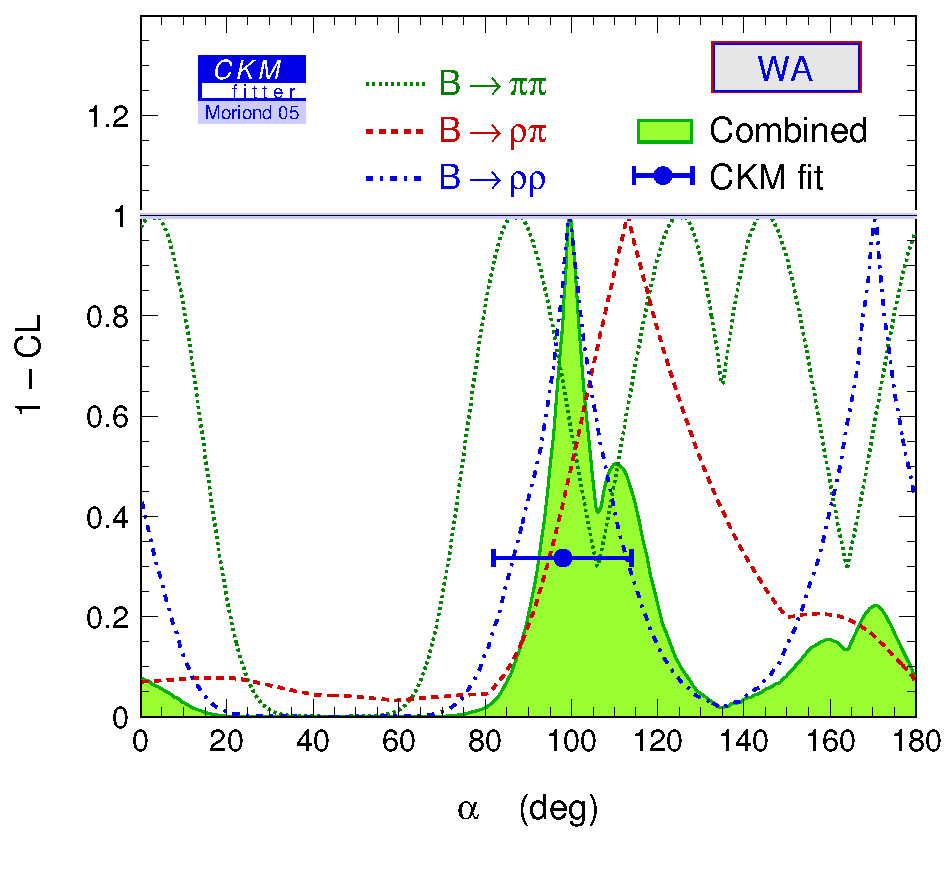
\includegraphics[width=\largefigwidth]{ckmfitter-alpha-combined}
%   \caption[CKM Fitter constraints on \alphaCKM.]%
%   {CKM Fitter constraints on \alphaCKM from combined \BToPiPi,
%     \BToRhoPi and \BToRhoRho decay analyses.}
%   \label{fig:CKMFitter}
% \end{figure}

\section{The \LHCb experiment}
\label{sec:LHCbInDetail}

Since both \bhadron{s} are preferentially produced in the same direction
and are forward-boosted along the beam-pipe, the detector is not required
to have full $4\pi$ solid-angle coverage. \LHCb takes advantage of this
by using a wedge-shaped single-arm detector with angular acceptance
\unit{10-300}{\mrad} in the horizontal (bending) plane~\cite{Amato:1998xt}.

\vspace{1cm}

\begin{center}
{\hspace{1mm}\Large\vdots\hspace{1cm}}
\end{center}

\vspace{1cm}

The detector is illustrated in \FigureRef{fig:LHCbCrossSection}, showing
the overall scale of the experiment and the surrounding cavern structure.

\begin{sidewaysfigure}
  \begin{center}
  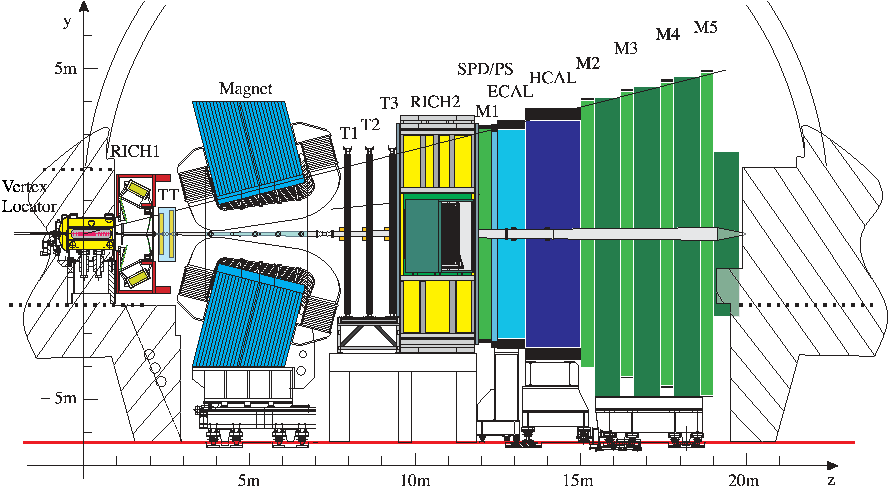
\includegraphics[width=0.8\textheight]{lhcb-detector-cross-section}
  \caption[Cross-section view of \LHCb, cut in the non-bending $y$--$z$ plane]%
    {Cross-section view of \LHCb, cut in the non-bending $y$--$z$ plane.}
  \label{fig:LHCbCrossSection}
  \end{center}
\end{sidewaysfigure}

The single-sided detector design was chosen in preference to a two-armed
design since the detector dimensions are restricted by the layout of the
IP8 (ex-Delphi) cavern in which \LHCb is located. Using all the available
space for a single-arm spectrometer more than compensates in performance
for the \about{50\percent} drop in luminosity.

\section{The \Cerenkov mechanism}
A Huygens construction in terms of spherical shells of probability for photon
emission as the particle progresses along its track shows an effective
``shock-front'' of \Cerenkov emission. This corresponds to an emission cone of
opening angle \thetaCerenkov around the momentum vector for each point on the
track,
%
\begin{subequations}
  \label{eq:cosThetaCk}
  \begin{equation}
    \cos\,\thetaCerenkov  &= \frac{1}{n \beta} +
                             \frac{\hbar k}{2p}%
                             \parenths{ 1 - \frac{1}{n^2} } \\
                          &\,\sim \frac{1}{n \beta}%
    \label{eq:cosThetaCkApprox}
  \end{equation}
\end{subequations}
%
where $\beta \equiv v/c$, the relativistic velocity fraction.

\section{Trigger system}
\label{sec:triggers}
An overview of the \LHCb trigger characteristics broken down by level
is shown in \Table~\ref{tab:TriggerDetails}.

\begin{table}[bp]
  \begin{tabular}{lllll}
                & L0              & L1              & HLT             \\
    \midrule\\
    Input rate  & \unit{40}{\MHz} & \unit{1}{\MHz}  & \unit{40}{\kHz} \\
    Output rate & \unit{1}{\MHz}  & \unit{40}{\kHz} & \unit{2}{\kHz}  \\
    Location    & On detector     & Counting room   & Counting room   \\
  \end{tabular}
  \caption{Characteristics of the trigger levels and offline analysis.}
  \label{tab:TriggerDetails}
\end{table}

  \chapter{Continued captions}
\label{chap:ContCaptions}

Here are some funky floats using ``continued captions'', i.e. for a semantically
collected group of float contents which are too numerous to fit into a single
float, such as the pretty circles in the following figure:

\newcommand{\circleimg}[1]{%
\begin{tikzpicture}
  \draw[color=black,fill=#1,thick] (1,0) circle (1.5cm);
\end{tikzpicture}%
}

\begin{figure}[hb]
  \subfloat[][Example 1a]{\label{fig:cc1a}\circleimg{red!80}}\quad
  \subfloat[][Example 1b]{\label{fig:cc1b}\circleimg{green!70!yellow}}\quad
  \subfloat[][Example 1c]{\label{fig:cc1c}\circleimg{blue!80}}\quad
  \subfloat[][Example 1d]{\label{fig:cc1d}\circleimg{orange!80!yellow}}
  \caption{Demonstration of \texttt{subfig} continued captions.}
  \label{fig:cc1}
\end{figure}

\begin{figure}[p]
  \ContinuedFloat
  \subfloat[][Example 1e]{\label{fig:cc1e}\circleimg{violet}}\quad
  \subfloat[][Example 1f]{\label{fig:cc1f}\circleimg{cyan}}\quad
  \subfloat[][Example 1g]{\label{fig:cc1g}\circleimg{magenta}}\quad
  \subfloat[][Example 1h]{\label{fig:cc1h}\circleimg{yellow}}
  \caption[]{Demonstration of \texttt{subfig} continued captions (continued).}
\end{figure}

\noindent
This mechanism means that the same float label is used for both pages of
floats. Note that we can refer to \FigureRef{fig:cc1} in general, or to
\FigureRef{fig:cc1g} on \PageRef{fig:cc1g} in particular!

\noindent
Just for the hell of it, let's also refer to \SectionRef{sec:neutralmixing}.

  %% To ignore a specific chapter while working on another, making the build faster, comment it out:
  %\input{chap4}
\end{mainmatter}

%% Produce the appendices
\begin{appendices}
  %% The "\appendix" call has already been made in the declaration
%% of the "appendices" environment (see thesis.tex).
\chapter{Pointless extras}
\label{app:Pointless}

\chapterquote{%
Le savant n'\'etudie pas la nature parce que cela est utile; \\
\indent il l'\'etudie parce qu'il y prend plaisir, \\
\indent et il y prend plaisir parce qu'elle est belle.}%
{Henri Poincar\'e, 1854--1912}

Appendixes (or should that be ``appendices''?) make you look really clever, 'cos
it's like you had more clever stuff to say than could be fitted into the main
bit of your thesis. Yeah. So everyone should have at least three of them\dots

\section{Like, duh}
\label{sec:Duh}
Padding? What do you mean?

\section{$y = \alpha x^2$}
\label{sec:EqnTitle}
See, maths in titles automatically goes bold where it should (and check the
table of contents: it \emph{isn't} bold there!) Check the source: nothing
needs to be specified to make this work. Thanks to Donald Arsenau for the
teeny hack that makes this work.

%% Big appendixes should be split off into separate files, just like chapters
%\input{app-myreallybigappendix}

\end{appendices}

%% Produce the un-numbered back matter (e.g. colophon,
%% bibliography, tables of figures etc., index...)
\begin{backmatter}
  \begin{colophon}
  This thesis was made in \LaTeXe{} using the ``hepthesis'' class~\cite{hepthesis}.
\end{colophon}

%% You're recommended to use the eprint-aware biblio styles which
%% can be obtained from e.g. www.arxiv.org. The file mythesis.bib
%% is derived from the source using the SPIRES Bibtex service.
\bibliographystyle{h-physrev}
\bibliography{mythesis}

%% I prefer to put these tables here rather than making the
%% front matter seemingly interminable. No-one cares, anyway!
\listoffigures
\listoftables

%% If you have time and interest to generate a (decent) index,
%% then you've clearly spent more time on the write-up than the 
%% research ;-)
%\printindex

\end{backmatter}

%% Close
\end{document}
